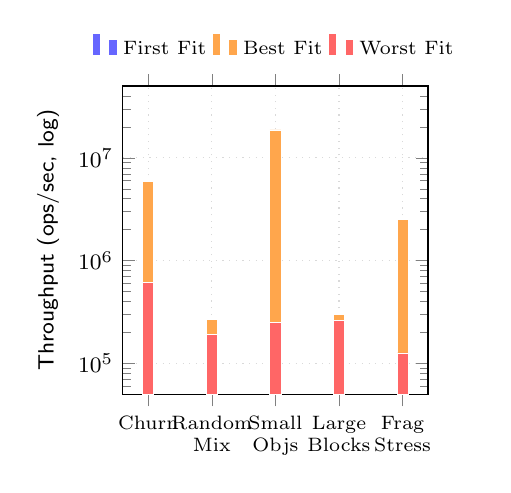
\begin{tikzpicture}[font=\footnotesize\sffamily]
\begin{axis}[
    width=0.45\textwidth, height=5.5cm,
    ybar, bar width=4pt,
    ymode=log, log origin=infty,
    ylabel={Throughput (ops/sec, log)},
    xtick=data,
    xticklabels={
Churn, {Random\\Mix}, {Small\\Objs}, {Large\\Blocks}, {Frag\\Stress}
},
    xticklabel style={align=center, text width=1.8cm, font=\scriptsize},
    ymin=50000, ymax=50000000,
    legend style={at={(0.5,1.05)}, anchor=south, legend columns=3, font=\scriptsize, draw=none},
    grid=major, grid style={dotted, gray!30},
    ymajorgrids=true,
    bar shift=0pt,
]

\addplot[fill=blue!60, draw=white, line width=0.3pt] coordinates {
  (1, 5272213)
  (2, 261050)
  (3, 18580661)
  (4, 249241)
  (5, 1019623)
};
\addlegendentry{First Fit}
\addplot[fill=orange!70, draw=white, line width=0.3pt] coordinates {
  (1, 5914130)
  (2, 269235)
  (3, 18666415)
  (4, 301535)
  (5, 2501066)
};
\addlegendentry{Best Fit}
\addplot[fill=red!60, draw=white, line width=0.3pt] coordinates {
  (1, 610266)
  (2, 190860)
  (3, 252052)
  (4, 264624)
  (5, 126723)
};
\addlegendentry{Worst Fit}
\end{axis}
\end{tikzpicture}
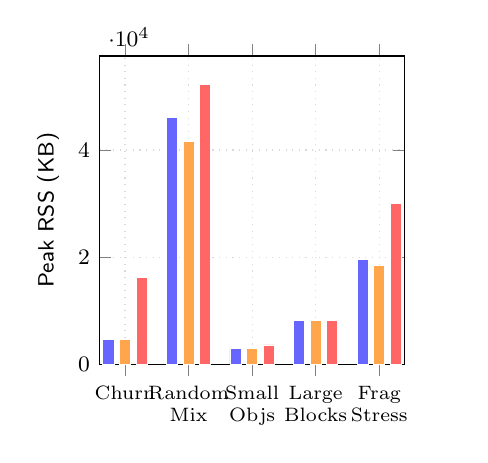
\begin{tikzpicture}[font=\footnotesize\sffamily]
\begin{axis}[
    width=0.45\textwidth, height=5.5cm,
    ybar, bar width=4pt,
    ylabel={Peak RSS (KB)},
    xtick=data,
    xticklabels={
Churn, {Random\\Mix}, {Small\\Objs}, {Large\\Blocks}, {Frag\\Stress}
},
    xticklabel style={align=center, text width=1.8cm, font=\scriptsize},
    ymin=0,
    legend style={at={(0.5,1.05)}, anchor=south, legend columns=3, font=\scriptsize, draw=none},
    grid=major, grid style={dotted, gray!30},
]

\addplot[fill=blue!60, draw=white, line width=0.3pt] coordinates {
  (1, 4680)
  (2, 46020)
  (3, 3016)
  (4, 8136)
  (5, 19524)
};
\addplot[fill=orange!70, draw=white, line width=0.3pt] coordinates {
  (1, 4644)
  (2, 41632)
  (3, 3016)
  (4, 8132)
  (5, 18500)
};
\addplot[fill=red!60, draw=white, line width=0.3pt] coordinates {
  (1, 16316)
  (2, 52292)
  (3, 3652)
  (4, 8136)
  (5, 30024)
};
\end{axis}
\end{tikzpicture}
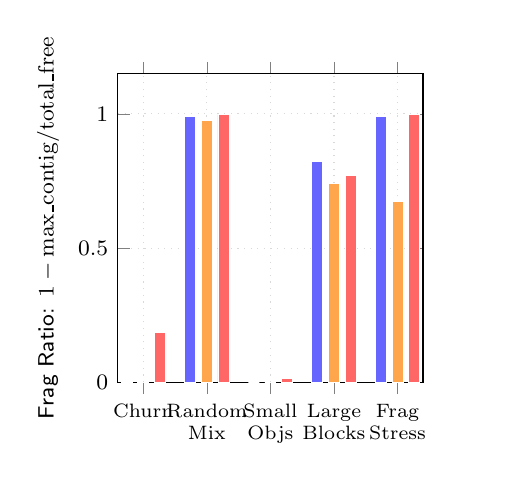
\begin{tikzpicture}[font=\footnotesize\sffamily]
\begin{axis}[
    width=0.45\textwidth, height=5.5cm,
    ybar, bar width=4pt,
    ylabel={Frag Ratio: $1 - \mathrm{max\_contig} / \mathrm{total\_free}$},
    xtick=data,
    xticklabels={
Churn, {Random\\Mix}, {Small\\Objs}, {Large\\Blocks}, {Frag\\Stress}
},
    xticklabel style={align=center, text width=1.8cm, font=\scriptsize},
    ymin=0, ymax=1.15,
    legend style={at={(0.5,1.05)}, anchor=south, legend columns=3, font=\scriptsize, draw=none},
    grid=major, grid style={dotted, gray!30},
]

\addplot[fill=blue!60, draw=white, line width=0.3pt] coordinates {
  (1, 0.0027)
  (2, 0.9917)
  (3, 0.0)
  (4, 0.8231)
  (5, 0.9918)
};
\addplot[fill=orange!70, draw=white, line width=0.3pt] coordinates {
  (1, 0.0006)
  (2, 0.9748)
  (3, 0.0)
  (4, 0.7396)
  (5, 0.6733)
};
\addplot[fill=red!60, draw=white, line width=0.3pt] coordinates {
  (1, 0.1845)
  (2, 0.997)
  (3, 0.0127)
  (4, 0.769)
  (5, 0.9975)
};
\end{axis}
\end{tikzpicture}